\documentclass[12pt,utf8]{beamer}
\setbeamercovered{transparent}
\usepackage[german]{babel}
\usepackage{color}
\usepackage{xcolor}
\usepackage{graphicx}
\usepackage{tikz}
\usetheme{FOSSAG}

\title{Linux Basics}
\subtitle{Das Terminal}


\author[J.-M. Lenk, C. Parnitzke, Y. Bungers, A. Becker]{Jan-Marius Lenk, Christoph Parnitzke, Yannick Bungers, Alexander Becker}
\institute[FOSS AG]{Free and Open Source Software AG\\ Fakultät für Informatik}

\date{\today}

\begin{document}

\titlepage

\begin{frame}
\frametitle{Inhaltsverzeichnis}
\begin{itemize}
	\item Einleitung
	\item Arbeiten mit Ordnern, Dateien und Archiven
	\item Systemverwaltung
\end{itemize}
\end{frame}

\section{Einleitung}
\begin{frame}
\frametitle{Unix Philosophie}
\begin{figure}

\includegraphics[scale=0.15]{res/tuX_tu.png}
\end{figure}
\begin{itemize}
	\item Philosophie besteht aus drei Punkten:
	\begin{itemize}
		\item 1. Schreibe Programme, die nur eine Sache tun und dies erfolgreich
		\item 2. Schreibe Programme, die Kolaboration ermöglichen
		\item 3. Schreibe Programme, die mit Text arbeiten, denn dies ist universell
	\end{itemize}
\end{itemize}
%\footnote{https://upload.wikimedia.org/wikipedia/commons/a/af/Tux.png}
\end{frame}

%autocompletion einfach erwähnen und als notiz auf Handout
%\begin{frame}
%\frametitle{Aufgabe 1}
%Nun sollt ihr euch ein wenig mit der \texttt{man}-Page und dem Paket-Management vertraut machen. Zur Bearbeitung dieser Aufgabe habt ihr 10 Minuten Zeit.
%\begin{itemize}
%	\item[1)] führt ein Update der Quellen durch; \texttt{apt update}
%	\item[2)] installiert das Paket \texttt{funny-manpages}
%	\begin{itemize}
%		\item benutzt dazu \texttt{apt install}
%		\item \texttt{sudo} nicht vergessen!!
%	\end{itemize}
%	\item[3)] betrachtet folgende \texttt{man}-Pages:
%	\begin{itemize}
%		\item \texttt{su}, \texttt{apt-get}, \texttt{party}, \texttt{t}, \texttt{tm}, \texttt{flog}
%	\end{itemize}
%	\item[4)] (optional) \texttt{funny-manpages} entfernen, wer mag
%	\begin{itemize}
%		\item benutzt dazu \texttt{apt remove}
%	\end{itemize}
%\end{itemize} 
%\end{frame}

\section{Arbeiten mit Ordnern, Dateien und Archiven}
\subsection{Ordner}
\begin{frame}
	\frametitle{\textcolor{lightGreen}{l}i\textcolor{lightGreen}{s}t}
	\framesubtitle{Ein kleines Licht in der Dunkelheit}
	\begin{itemize}
		\item Listet alle Ordner und Dateien in Verzeichnis auf
		\item Mögliche Optionen:
		\begin{itemize}[<+->]
			\item \texttt{-a}  (all) inkl. versteckter Verzeichnisse
			\item \texttt{-hl}  (human readable / long listing format) inkl. Rechte, Besitzer, Größe, etc.
		\end{itemize}
	\end{itemize}
\end{frame}

\begin{frame}
	\frametitle{\textcolor{lightGreen}{c}hange \textcolor{lightGreen}{d}irectory}
	\framesubtitle{Die kleine Form der Teleportation}
	\texttt{cd} ermöglicht das Navigieren durch das Dateisystem
	\begin{itemize}
		\item Wechsel in Parent-Directory mit \texttt{cd ..}
		\item Wechsel in Home-Directory mit \texttt{cd} ($\sim$)
	\end{itemize}
\end{frame}

\begin{frame}
	\frametitle{find}
	\texttt{find} sucht Dateien im aktuellen Ordner und in Unterordnern
	\begin{itemize}
		\item \texttt{find -name FILE}
	\end{itemize}
\end{frame}

\begin{frame}
\frametitle{\textcolor{lightGreen}{m}a\textcolor{lightGreen}{k}e \textcolor{lightGreen}{dir}ectory}
\framesubtitle{Verzeichnisse erschaffen}
\texttt{mkdir} erstellt Ordner auf dem Rechner
\begin{itemize}
	\item \texttt{mkdir PATH}
	\item \texttt{-p} erstellt alle Ordner auf dem Pfad, die noch nicht existieren
\end{itemize}
\end{frame}

%\begin{frame}
%\frametitle{Aufgabe 2)}
%In der zweiten Aufgabe sollt ihr euch mit der Verwaltung von Ordnern beschäftigen. Zur Bearbeitung stehen euch 15 Minuten zur verfügung.
%{\footnotesize
%\begin{itemize}
%	\item wechselt in das Verzeichnis \texttt{/tmp}
%	\item erstellt den Ordner \texttt{test}
%	\item guckt euch die Rechte des Ordners an
%	\item entfernt die Rechte für \texttt{group} und \texttt{other} des Ordners
%	\item setzt als neuen Owner des Ordners \texttt{root} \texttt{[nur Root]}
%	\item versucht den Ordner zu entfernen (ohne \texttt{sudo}). Was passiert?
%	\item wechselt nun wieder den Owner zurück \texttt{[nur Root]}
%	\item entfernt den Ordner
%\end{itemize}
%}
%{\scriptsize Tipp: \texttt{cd}, \texttt{ls}, \texttt{mkdir}, \texttt{chmod}, \texttt{chown}, \texttt{rmdir}}
%\end{frame}

\subsection{Dateien}
\begin{frame}
	\centering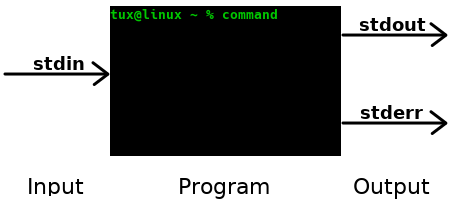
\includegraphics[scale=0.65]{res/IOE}
\end{frame}

\begin{frame}
	\Huge\centering{$|$~~~$>$}
\end{frame}

%\begin{frame}
%	\frametitle{con\textcolor{lightGreen}{cat}enate}
%	\framesubtitle{Was eine Katze mit Linux zu tun hat}
%	\texttt{cat} konkateniert und zeigt die Inhalte von Dateien
%	\begin{itemize}
%		\item An sich nicht mächtig, sehr einfacher Befehl
%		\item Parameter (Default: -u):
%		\begin{itemize}[<+->]
%			\item \texttt{-n} Nummeriert die ausgegebenen Zeilen 
%			\item \texttt{-e} Fügt am Ende jeder Zeile ein \$ hinzu
%		\end{itemize}
%		\item Bsp.: \texttt{cat -n output.txt output2.txt}
%	\end{itemize}
%\end{frame}

\begin{frame}
\frametitle{\Large Dateien betrachten und bearbeiten}
\begin{itemize}
	\item \texttt{cat FILE} - Ausgabe einer Datei
	\item \texttt{less FILE} - Betrachten einer Datei
	\item \texttt{nano FILE} - Bearbeiten einer Datei
\end{itemize}
\end{frame}

\begin{frame}
	\frametitle{\Large{\textcolor{lightGreen}{g}lobally search a \textcolor{lightGreen}{r}egular \textcolor{lightGreen}{e}xpression and \textcolor{lightGreen}{p}rint}}
	\framesubtitle{Gonna catch em' Strings}
	\texttt{grep} ermöglicht die Suche in einer Eingabe
	\begin{itemize}
		\item \texttt{-i} ignoriert Groß- und Kleinschreibung bei der Suche
	\end{itemize}
\end{frame}

%\begin{frame}
%	\frametitle{\textcolor{red}{g}lobally search a \textcolor{red}{re}gular expression and \textcolor{red}{p}rint}
%	\framesubtitle{\textcolor{ownDarkOr}{Gonna catch em' Strings}}
%	Durchsucht eine Eingabe nach einem RegEx.\\
%	Der Name kommt von den Befehlen g, re und p aus dem Editor Ed
%	Default: -G
%	{\footnotesize
%		\begin{table}
%			\begin{tabular}{l c}
%				
%				\begin{tabular}{l|c}
%					&{\scriptsize \textbf{Selektoren}} (interpretieren Suchwort als)\\
%					\hline
%					\textbf{\textcolor{ownDarkOr}{\texttt{-E}}} & erweiterter RegEx \\
%					\hline
%					\textbf{\textcolor{ownDarkOr}{\texttt{-F}}} & fixed String\\
%					\hline 
%					\textbf{\textcolor{ownDarkOr}{\texttt{-G}}} & basic RegEx\\
%					
%				\end{tabular} \\ \\
%				\begin{tabular}{l|c}
%					& {\scriptsize \textbf{Ausgabe}}\\
%					\hline
%					\textbf{\textcolor{ownDarkOr}{\texttt{-c}}} & Anzahl passender Zeilen\\
%					\hline
%					\textbf{\textcolor{ownDarkOr}{\texttt{-o}}} & nur gematchte Teile einer Zeile\\
%					\hline
%					\textbf{\textcolor{ownDarkOr}{\texttt{-q}}} & keine Ausgabe, nur Exitcode  \\
%					& (0 wenn erfolgreich)\\
%				\end{tabular}
%				&
%				\begin{tabular}{l|c}
%					& {\scriptsize \textbf{Kontrolle}}\\
%					\hline
%					\textbf{\textcolor{ownDarkOr}{\texttt{-f [file]}}} & liest RegEx aus [file]\\
%					\hline
%					\textbf{\textcolor{ownDarkOr}{\texttt{-v}}} & invertiert Matchmaking\\
%					\hline
%					\textbf{\textcolor{ownDarkOr}{\texttt{-w}}} & nur Zeilen, in denen ganze\\
%					& Worte RegEx entsprechen\\ 
%					\hline
%					\textbf{\textcolor{ownDarkOr}{\texttt{-x}}} & nur Zeilen, die ganz \\
%					& dem RegEx entsprechen \\
%				\end{tabular} 
%				
%			\end{tabular}
%		\end{table}
%	}
%\end{frame}

%\begin{frame}
%	\frametitle{nano}
%	Ermöglicht das bearbeiten von Textdateien im Terminal.
%	\begin{itemize}
%		\item minimalistisch
%		\item leichte Bedienung
%		\item bietet alle Standardfunktionen eines Texteditors
%	\end{itemize}
%	Umfangreichere Alternative stellt \texttt{vim} dar.
%\end{frame}

%\begin{frame}
%	\frametitle{Texteditoren - 1: \texttt{ed}, \texttt{nano}, \texttt{pico}}
%	\framesubtitle{\textcolor{ownDarkOr}{You would (not) love Ed!!}}
%	Das Bearbeiten von Textdateien ist in der Konsole schwierig. Ein Beispiel ist \texttt{ed} (release 1970; Grundlage für \texttt{grep}).
%	\begin{itemize}
%		\item \texttt{pico} (release 1992):
%		\begin{itemize}[<+->]
%			\item {\scriptsize sehr minimalistischer Editor}
%			\item {\scriptsize reine Textverarbeitung, mehrere Dokumente möglich, Syntaxhighlighting}
%			\item {\scriptsize kein Highlighting Wörtern, kein Text-Splitscreen, keine RegEx-Suche}
%		\end{itemize}
%		\item \texttt{nano} (release 1999):
%		\begin{itemize}[<+->]
%			\item {\scriptsize ebenfalls sehr minimalistisch}
%			\item {\scriptsize Nachfolger von \texttt{pico}}
%			\item {\scriptsize bietet mehr Funktionsumfang, z.B.: Text-Splitscreen, RegEx-Suche}
%		\end{itemize}
%		\item \texttt{nano} und \texttt{pico} sind sehr minimalistisch, aber nicht zu unterschätzen
%	\end{itemize}
%\end{frame}
%
%\begin{frame}
%	\frametitle{Texteditoren - 2: \texttt{vim}, \texttt{jed}}
%	\framesubtitle{\textcolor{ownDarkOr}{Good thing Ed is not around anymore}}
%	Wir haben grad die minimaltistischen Editoren betrachtet, nun die etwas mächtigeren.
%	\begin{itemize}
%		\item \texttt{vim} (release 1991):
%		\begin{itemize}[<+->]
%			\item Großmufti unter den Editoren
%			\item verbesserte Suchfunktionen, mächtiger als \texttt{nano} und \texttt{pico}
%			\item Standard bei \texttt{git}
%		\end{itemize}
%		\item \texttt{jed} (release 1992):
%		\begin{itemize}[<+->]
%			\item \textbf{der} Editor für Programmierer
%			\item liefert Templates für verschiedene Anwendungsfälle
%			\item weniger mächtig als \texttt{vim}, aber dennoch viele Features
%		\end{itemize}
%		\item Bei der Wahl des Editors ist es wie immer im Leben, Geschmäcker sind verschieden
%	\end{itemize}
%\end{frame}

%\begin{frame}
%\frametitle{Aufgabe 3)}
%In dieser Aufgabe sollt ihr euch mit der Umleitung der Standardausgabe beschäftigen. Für die Bearbeitung habt ihr 5 Minuten.
%\begin{itemize}
%	{\footnotesize
%	\item wechselt in euer Home-Verzeichnis
%	\item lasst euch die Inhalte reversiv ausgeben
%	\item benutzt die Ausgabe als Eingabe für \texttt{cowsay} (Pipe-Operator)
%	\item lasst euch nun diese Ausgabe in die Datei \texttt{KuhSagtHome.txt} schreiben
%	\item seht euch den Inhalt der Datei an
%	}
%\end{itemize}
%{\scriptsize Tipp: \texttt{cd}, \texttt{ls}, \texttt{cowsay}, \texttt{$\mid$}, \texttt{>}, \texttt{less}}
%\end{frame}

\begin{frame}
\frametitle{\textcolor{lightGreen}{c}o\textcolor{lightGreen}{p}y $\&$ \textcolor{lightGreen}{m}o\textcolor{lightGreen}{v}e}
\framesubtitle{Die Kunst des Klonens und Umbenennens}
\begin{itemize}
	\item \texttt{mv PATH1 PATH2} (Verschieben von Dateien/Ordnern)
	\item \texttt{cp PATH1 PATH2} (Kopieren von Dateien)
	\begin{itemize}
		\item -r ermöglicht kopieren von Ordnern
	\end{itemize}
\end{itemize}
\end{frame}

\begin{frame}
\frametitle{\textcolor{lightGreen}{r}e\textcolor{lightGreen}{m}ove}
\framesubtitle{Flutsch! Und weg!}
\begin{itemize}
	\item \texttt{rm [OPTION] FILE}
	\begin{itemize}[<+->]
		\item \texttt{-r} ermöglicht das Löchen von Ordnern
	\end{itemize}
\end{itemize}
\end{frame}

%\begin{frame}
%\frametitle{Aufgabe 4)}
%Diese Aufgabe soll euch ein Gefühl für den Umgang mit Dateien geben. Für die Bearbeitung habt ihr 15 Minuten.
%\begin{itemize}
%	{\footnotesize
%	\item lasst euch alle Dateien in \texttt{/usr/share} ausgeben, die dem folgenden RegEx entsprechen \texttt{".*.txt"} und schreibt die Ausgabe in \texttt{/home/[username]/txt-files.txt}
%	\item schaut euch nun den Inhalt an
%	\item sucht nach eurer Datei \texttt{KuhSagtHome.txt} und schreibt das Ergebnis in \texttt{kuh-sagt-path.txt} (Suche in \texttt{/home})
%	\item verbindet nun den Inhalt von \texttt{txt-files.tx}' und \texttt{kuh-sagt-path.txt} und schreibt die Ausgabe in \texttt{cat-files-kuh.txt}
%	\item betrachtet das Ende der Datei \texttt{cat-files-kuh.txt}. Was fällt auf?
%	\item sortiert den Inhalt von \texttt{cat-files-kuh.txt} numerisch und schreibt die Ausgabe in \texttt{sort-cat-kuh.txt}
%	\item betrachtet den Anfang von \texttt{sort-cat-kuh.txt}. Was hat sich verändert?
%	\item löscht nun alle eben erstellten Dateien
%	}
%\end{itemize}
%{\scriptsize Tipp: \texttt{find}, \texttt{less} bzw. \texttt{more}, \texttt{cat}, \texttt{tail}, \texttt{head}, \texttt{sort}, \texttt{rm} bzw. \texttt{shred}}
%\end{frame}


\subsection{Archive}
\begin{frame}
\frametitle{\textcolor{lightGreen}{t}ape \textcolor{lightGreen}{ar}chiver}
\framesubtitle{Archivieren}
Zum entpacken von Archiven wie \texttt{.tar}, \texttt{.tar.gz}, \texttt{.zip}, etc. 
\begin{itemize}
	\item \texttt{tar -czvf ARCHIVE\_PATH PATH\_FILES}\\(Verpacken)
	\item \texttt{tar -xzvf ARCHIVE\_PATH}\\(Entpacken)
\end{itemize}
\end{frame}

\begin{frame}
\frametitle{\textcolor{lightGreen}{t}ape \textcolor{lightGreen}{ar}chiver}
\framesubtitle{Archivieren}
	\begin{itemize}[<+->]
		\item {\scriptsize \texttt{-c} (create) erzeugt neues Archiv}
		\item {\scriptsize \texttt{-x} (extract) extrahieren einer Datei}
		\item {\scriptsize \texttt{-v} (verbose) Fortschritt auflisten}
		\item {\scriptsize \texttt{-z} (gzip format) komprimieren als \texttt{.gz}, etc.}
		\item {\scriptsize \texttt{-f} erzeugt beim Entpacken einen Ordner mit Namen von Archiv}
	\end{itemize}
\end{frame}

\section{Systemverwaltung}
\subsection{Prozesse verwalten}
\begin{frame}
\frametitle{\textcolor{lightGreen}{h}isham \textcolor{lightGreen}{t}able \textcolor{lightGreen}{o}f \textcolor{lightGreen}{p}rocesses}
\framesubtitle{interaktiver Prozessmanager}
\begin{itemize}
	\item \texttt{\textcolor{red}{t}able \textcolor{red}{o}f \textcolor{red}{p}rocesses} (bereits installtiert)
	\item \texttt{htop} (muss installiert werden)
	\begin{itemize}[<+->]
		\item {\scriptsize Übersicht über alle Prozesse und verbrauchte Ressourcen}
		\item {\scriptsize deutlich leichtere Bedienung und bessere Übersicht}
		\item {\scriptsize bietet mehr Interaktionen}
	\end{itemize}
\end{itemize}
\end{frame}

\begin{frame}
	\Huge\centering{\&}
\end{frame}

%\subsection{IP-Adressen}
%\begin{frame}
%	\frametitle{ip addr}
%	Meist wurde \texttt{ifconfig} benutzt um sich seine lokalen IP-Adressen des Rechners anzeigen zu lassen. Dieser Befehl ist allerdings ein wenig obsolet und wurde ersetzt durch \texttt{ip addr}.
%	\begin{itemize}
%		\item Um lokale IP-Adresse zu erfahren, ohne über Router zu gehen
%		\item leider etwas unübersichtlich
%		\begin{itemize}
%			\item {\scriptsize Gegenmaßnahme: \texttt{ip addr $\mid$ grep inet}}
%		\end{itemize}
%	\end{itemize}
%\end{frame}

\subsection{Paketverwaltung}
\begin{frame}
	\frametitle{\textcolor{lightGreen}{s}uper \textcolor{lightGreen}{u}ser \textcolor{lightGreen}{do}}
	\framesubtitle{Mit großer Macht kommt große Verantwortung}
	\texttt{sudo} führt einen Befehl mit administrativer Berechtigung aus
	\begin{itemize}
		\item \texttt{sudo COMMAND}
	\end{itemize}
\end{frame}

\begin{frame}
	\frametitle{apt}
	Mit \texttt{apt} lassen sich Pakete installieren und deinstallieren
	\begin{itemize}
		\item \texttt{sudo apt install PACKAGE}
		\item \texttt{sudo apt update}
		\item \texttt{sudo apt upgrade / dist-upgrade}
		\item \texttt{sudo apt remove PACKAGE}
		\item \texttt{sudo apt search PACKAGE}
	\end{itemize}
\end{frame}

\begin{frame}
	\frametitle{man page}
	\framesubtitle{Wenn man mal nicht weiter weiß}
	Anleitungen (Manuals) zu den installierten Paketen lassen sich mit \texttt{man} betrachten.
	\begin{itemize}
		\item man COMMAND
	\end{itemize}
\end{frame}

%\begin{frame}
%\frametitle{Aufgabe 5)}
%In dieser Aufgabe sollt ihr euch mit der Verwaltung von Prozessen beschäftigen.
%Für die Bearbeitung stehen euch 10 Minuten zur Verfügung.
%\begin{itemize}
%	{\footnotesize
%	\item ladet euch die Datei \texttt{infinite.tar} von \texttt{foss-ag.de} herunter
%	\item verschiebt sie nach \texttt{/tmp} und entpackt sie dort
%	\item führt den Befehl \texttt{python infinite$\_$run.py} im Hintergrund aus mit Nice-Wert 15
%	\item führt \texttt{htop} bzw. \texttt{top} aus, sucht euren Prozess und merkt euch die \texttt{PID}
%	\item verändert den Nice-Wert auf 10 und schaut in \texttt{htop} bzw. \texttt{top} nach, was passiert ist
%	\item stoppt nun den Prozess mit dem Befehl \texttt{kill}, wobei ihr die \texttt{PID} angeben müsst
%	}
%\end{itemize}
%{\scriptsize Tipp: \texttt{tar}, \texttt{mv}, \texttt{nice}, \texttt{\&}, \texttt{renice}, \texttt{htop} bzw. \texttt{top}}
%\end{frame}

\subsection{Herunterfahren und Neustarten}
\begin{frame}
\frametitle{poweroff und reboot}
\framesubtitle{Wenn man mal das real life genießen will}
\begin{itemize}
	\item \texttt{poweroff} (Herunterfahren des Systems)
	\item \texttt{reboot} (Neustart des Systems)
\end{itemize}
\end{frame}

%\begin{frame}
%\frametitle{Aufgabe 6)}
%Diese Aufgabe soll euch ein Gefühl für RegEx geben.
%\begin{itemize}
%{\footnotesize
%	\item lasst euch eure IP-Adresse ausgeben und schreibt die Ausgabe in \texttt{ip.txt}
%	\item lasst euch nun nur die Zeilen Ausgeben, die eine valide IP-Adresse enthalten (IPv4, IPv6, oder beides)
%	\item \textbf{Achtung!!} es gibt mehrere Lösungen
%	}
%\end{itemize}
%{\scriptsize Tipp: \texttt{ip addr}, \texttt{grep}, \texttt{RegEx}}
%\end{frame}

\end{document}
